\documentclass[11pt]{article}

\usepackage[T1]{fontenc}
\usepackage{mathptmx}
\usepackage{graphicx}

\topmargin 0.0in
\setlength{\textwidth} {420pt}
\setlength{\textheight} {620pt} 
\setlength{\oddsidemargin} {20pt}
\setlength{\marginparwidth} {72in}

\usepackage{fancyhdr} 
\usepackage{url}

% set it so that subsubsections have numbers and they
% are displayed in the TOC (maybe hard to read, might want to disable)

\setcounter{secnumdepth}{3}
\setcounter{tocdepth}{3}

% define widow protection

\def\widow#1{\vskip #1\vbadness10000\penalty-200\vskip-#1}

\clubpenalty=10000  % Don't allow orphans
\widowpenalty=10000 % Don't allow widows

% this should give me the ability to use some math symbols that 
% were available by default in standard latex (i.e. \Box)

\usepackage{latexsym}

% define a little section heading that doesn't go with any number

\def\littlesection#1{
\widow{2cm}
\vskip 0.5cm
\noindent{\bf #1}
\vskip 0.0001cm 
}

\pagestyle{fancyplain}

\newcommand{\tstamp}{\today}   
\renewcommand{\sectionmark}[1]{\markright{#1}}
\lhead[\Section \thesection]            {\fancyplain{}{\rightmark}}
\chead[\fancyplain{}{}]                 {\fancyplain{}{}}
\rhead[\fancyplain{}{\rightmark}]       {\fancyplain{}{\thepage}}
\cfoot[\fancyplain{\thepage}{}]         {\fancyplain{\thepage}{}}

\newlength{\myVSpace}% the height of the box
\setlength{\myVSpace}{1ex}% the default, 
\newcommand\xstrut{\raisebox{-.5\myVSpace}% symmetric behaviour, 
  {\rule{0pt}{\myVSpace}}%
}

% leave things with no spacing extra spacing in the final version of the paper
\renewcommand{\baselinestretch}{1.0}    % must go before the begin of doc

% suppress the use of indentation for a paragraph

\setlength{\parindent}{0.0in}
\setlength{\parskip}{0.1in}
\setlength{\headheight}{15pt}

\begin{document}

%% \begin{abstract}

%%   Try

%% \end{abstract}

% handle widows appropriately
\def\widow#1{\vskip #1\vbadness10000\penalty-200\vskip-#1}

% build the title section

\makeatletter

\def\maketitle{%
  %\null
  \thispagestyle{empty}%
  %\vfill
  \begin{center}%\leavevmode
    %\normalfont
    {\Huge \@title\par}%
    %\hrulefill\par
    {\normalsize \@author\par}%
    \vskip .4in
%    {\Large \@date\par}%
  \end{center}%
  %\vfill
  %\null
  %\cleardoublepage

  }

\makeatother

\vspace*{-1.1in}
\title{Pointer Based File Manager to Reduce Data Redundancy and Storage Costs}

% build the author section
\author{Braden D. Licastro\\
Department of Computer Science\\
Allegheny College \\
{\tt licastb@allegheny.edu}  \\
\url{http://www.fullforceapps.com/} \\ 
\vspace*{.1in} \today \\ \vspace*{.1in}
{\bf Abstract} \\ File sharing websites must overcome many hurdles to reliably operate with users submitting data continuously. Technologies have been implemented which limit the number, type, and size of the submitted files. Though these systems can be paired with file expiration times and other various systems, storage and backup costs remain high. To address this problem the research aims to create a pointer based environment that allows files to be accessed easily without creating unnecessary redundancy. Reducing the number of duplicate files benefits the business and the user in numerous ways, from faster response to decreased costs of storage and backups this issue is relevant on numerous fields.}

% use the default title stuff
\maketitle

\vspace*{-.4in}
\section{Introduction}
\label{sec:introduction}
\vspace*{-.1in}

Computers are absolutely everywhere, and society is becoming more digitized every day creating a need for storage of large amount of files. When running a website, storage space is at a premium, and the physical disks in the servers being used may not be local, but may in fact be located around the world. By allowing user submitted data, it quickly becomes apparent that data redundancy reduction can save a significant amount of storage space. This research will target the problem of data redundancy and provide a solution that will reduce not only storage costs but also inefficiencies. An implementation of a file management system will be introduced that is capable of managing large volumes of files using a database of location pointers and hash keys that identify each individual file. By using pointers, it is possible for the files to be stored on one central location or distributed across several systems while avoiding long search times.

By using text based entries in a database, a hashing function can be implemented which is capable of producing a unique hash code for each file in the collection. Because this key is unique for each different file, it is a reliable gauge of uniqueness. When multiple files are found to be identical only one physical copy will be kept but pointers to the database entry will allow easy access. On large, distributed network storage servers, the benefits become ever more apparent. As users store files on the disks, the system will hash each file and search for a match in a database, thus allowing the user access to the data, but eliminating the overhead of storing numerous copies of identical data. An increase in computation time will exist but should be minimal as text comparisons will be the primary task in finding uniqueness, but this will be outweighed by minimized physical storage requirements and costs of data backup.

The implementation of this system could be used in tandem with other currently implemented methods of file space cost reduction technologies out of the box. By not only using the proposed method of space requirement reduction, it could in theory be possible that with data expiration times, file size maximums, and similar technologies, that storage needs will plateau after the initial surge of additions and the expiration time has passed for the earliest uploaded file. This would allow webmasters to better predict overall needs and better predict upload trends and react accordingly with preventative maintenance and any required space additions.

\vspace*{-.1in}
\section{Related Work}
\label{sec:relatedwork}
\vspace*{-.1in}

A significant amount of work exists revolving around data optimization, but the idea of using databases of pointers and hashes to track file location on disk and file uniqueness is mostly undocumented. In addition to a mostly unexplored area of research, many of the data de-duplication methods are very costly when operating on large data sets. The first article to note addresses this issue. The authors set about creating a comparison and detection algorithm that is both fast and efficient. The authors utilized TI-Similarity and RAR methods for quickly scanning the database for potential duplicate records. \cite{Sung} When a duplicate entry is located it is removed from the collection.

\begin{figure}
\begin{center}
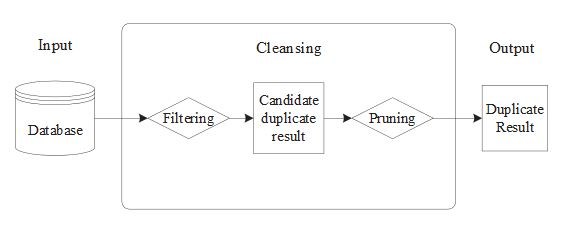
\includegraphics[scale=.8]{duplicate}
\caption{\label{fig:duplicate} The authors' filtering and pruning process.}
\end{center}
\end{figure}

As seen in figure \ref{fig:duplicate}, the database is input into the authors' program and the algorithm searches through the data looking for duplicates. Any duplicate results are evaluated and checked for false positives using the TI-Similarity method. \cite{Sung} Once a duplicate is validated, the result will be dropped from the database  and the resulting table will be returned and the database state will reflect the changes.

This method of finding duplicate data could be applied to the pointer based file system. By utilizing the authors' RAR and TI-Similarity search methods, it would be more efficient than searching the database one record at a time. The authors used an example table where identical data is inserted into a table by several users. As each entry has its own unique primary key value, the schema was satisfied, but the storage overhead is double what would be needed without redundancy. As seen in figure \ref{fig:duptable} there are three identical entries, their algorithm will remove all but the first occurrence leaving the end result of only rows $A$ and $D$.

\begin{figure}
\begin{center}
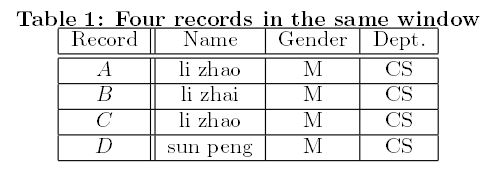
\includegraphics[scale=.8]{duptable}
\caption{\label{fig:duptable} Duplicate entries in the database to be removed.}
\end{center}
\end{figure}

The methods used by the authors could provide a solid foundation for the work being proposed. By adapting the comparison algorithms they used to work work with the system planned, it would create a more robust environment for file storage it could be possible to ensure that similar but different files are not falsely identified as identical and removed. Their algorithms cover not only the file itself, but they also look at the contents within it, mainly because it is capable of searching through databases for duplicate entries, which may include anything from plain text to blob objects. 

The next authors target the process of removing duplicate files from the physical disk itself. Throughout the paper, they create a framework for finding and removing duplicate file entries located on solid state drives. \cite{Wu} This is extremely valuable for not only the proposed research, but for any real world environment. Solid state drives have a limited number of writes per block of memory, by reducing the number of write requests, not only is the longevity of the disk being improved, but the total consumed space is also reduced therefore allowing more unique data per disk. Solid state drives are inherently fast, so it is possible that the framework, being optimized for said devices, could prove to be highly inefficient on traditional platter based disk drives. The authors track duplicates by the number of references made per file.

\begin{figure}
\begin{center}
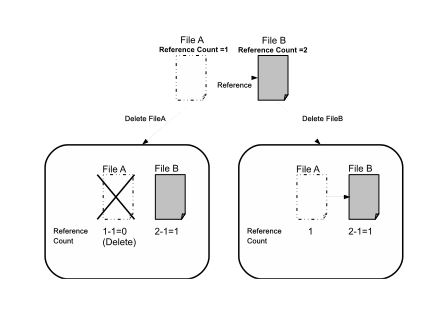
\includegraphics[scale=.8]{delete}
\caption{\label{fig:delete} Authors' file deletion process.}
\end{center}
\end{figure}

As seen in figure \ref{fig:delete}, if a file has a reference count of 0 it will be deleted. If the count is above 0, it cannot be removed as it is still referenced by another file or it is unique. If another file references an older version, the older version will be removed as the latest revision contains the contents of the old file. This method of removal us used in conjunction with perfect matches, as a perfect match is an exact duplicate. The latest modified instance of one of these files is kept, while others are rejected, or if already on disk, will be removed.

Although this research may not be a feasible method of redundancy reduction for the situation this research will address, sections of their research, data, and encountered troubles will be relevant. Due to the fact that the proposed research will be emulating a file sharing website, which could be located on one server, or distributed across a cluster of servers, the process of tracking files and eliminating duplicates becomes more difficult. The authors' process of finding duplicate blocks is applicable due to the fact that their methods were not restricted to a single system, but in fact were able to extend to any number of interconnected systems. This section of their research will be directly related to the proposed method of research as the storage system to be tested will include multiple nodes.

Several papers discuss the issue of bloated data backups due to duplicate data, but one specifically targets the reduction of duplicate data while the others focus on compression methods that enable algorithms to temporarily remove duplicates to reduce the archive size after completion of the backup. In the paper "Multi-level Comparison of Data Deduplication in a Backup Scenario", the authors focus on block level data redundancy elimination. This method is capable of pulling blocks out of a data stream and quickly finding exact matches already on disk in hopes to reduce archival storage needs or to reduce network traffic during said backups. \cite{Meister} After evaluating the final results of their research, the authors released their space savings as seen in figure \ref{fig:save}. These numbers are staggering, and in face go to show that even with 1-2\% of data being duplicate it is possible to reduce space overhead by a significant amount.

\begin{figure}
\begin{center}
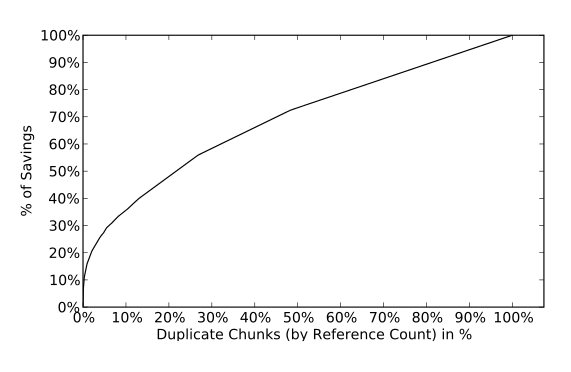
\includegraphics[scale=.7]{savings}
\caption{\label{fig:save} Results of the authors' data storage cost reduction methods.}
\end{center}
\end{figure}

Although these numbers may be staggering, the results were based off of block level reduction while the proposed research, as stated, will be comparing whole files. The authors did in fact use an identical method to what has been proposed to calculate whether a block is an exact match or not. To compute this result, the authors implemented a numeric hashing function that would create a 48 byte hash string representation of the data held in the blocks. From there, any matching 5-bit strings could be eliminated as an exact match. One difficulty with this process is identical data offset over several blocks of data. The authors addressed this by implementing a shifting function that would rotate the hashed block string using an alphabetic marker as a placeholder for where the shift began. If after shifting, a match was found, it then could be successfully removed. There is a draw back to this method though. As seen in figure \ref{fig:shift}, the authors encountered a scenario where shifting the data in either direction could result in a match in data. Shifting in one direction can lead to a one bit loss of characters in a string, while the other direction would prevent such a loss, but would cause a one bit remainder after duplicate data was removed and shifting completed. The authors were  able to resolve this issue by completing the reduction by replacing the missing characters with 0-values so shifting can continue across the next series of blocks.

\begin{figure}
\begin{center}
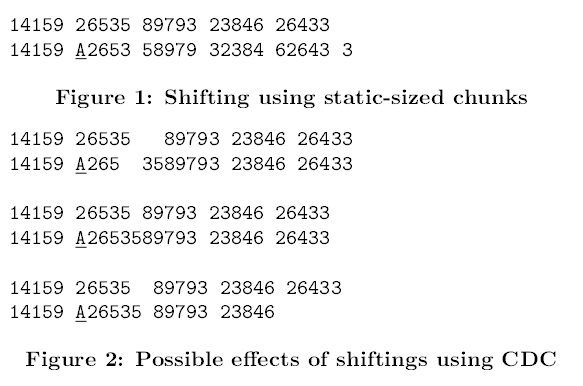
\includegraphics[scale=.7]{chunk_shift}
\caption{\label{fig:shift} Errors created by adding alphabetic placeholder and shifting hashed block values.}
\end{center}
\end{figure}

The next relevant paper will provide a method of searching file contents for duplicate entries, which could be used to infiltrate files and check for exact matches before removal in the proposed research. By hashing a file, it is assumed that every hash will be unique. There are a minimal number of cases where the hash of a file may be returned as an identical match, but in fact the two files may contain vastly different contents. The research would allow not only the hashing of a file, but content examination to insure that the file match in question is in fact a true match. The authors specifically addressed the issue of duplicate elimination for large data files, in which it is very common for duplicate entries to exist \cite{Bitton}. To reduce the number of file comparisons, the authors decided to sort all files by their file size and only compare those close in size. This would greatly reduce the number of comparisons and would also eliminate files that would not be a match given the file size is significantly different.

Finally, one of the most promising research papers gathered was a network storage system coined "Venti" developed by Bell Labs. This system was designed to be operated on a network and would be able to manage multiple nodes of data storage at a block level. \cite{Quinlan} The Venti storage system was developed to be used primarily as a means of reducing data storage costs in archival situations by using hashes of blocks of data as pointers and reducing the total number of identical blocks. \cite{Quinlan}

The working mature of the Venti system only allows for one write to each block, and because each block has a 160-bit SHA-1 hash of the contents, it was said that no other block could be found with the same address. When this algorithm was created, this may have been assumed true, but recently it has been proven otherwise. The file system works by assigning a hash "address" to each individual block, and once written to disk, it is considered permanent. When additional data was to be added to the system, the program would break the new data into blocks, create a hash for the item, and if it was unique, would then write it permanently to the archive as the data was not duplicate. Because the hashing function used is now considered insecure and is possible to get false positives, it is not a top contender for use in the proposed research. I would be implementing an SHA2-256 bit encryption method to ensure that no false positives would occur as it would be required to have a total of $2^2048$ files before a duplicate hash would be issued.

The Venti project will be useful in many ways; first, by looking at their system for storing the files and comparing hash es efficiently to find duplicates, it will be possible to use out of the box ,or optimize a method that has been tried and tested. In addition, the hashing algorithm and distributed file storage will be useful as those two features will be directly implemented into the proposed research. As seen in figure \ref{fig:venti}, Venti appears very similar to a web based network structure. There are users interacting through a network, which can be internal, or over the internet, and internally Venti checks the blocks against a block cache, then locates the hash index and block location on disk and finally either retrieves the data or stores the unique new blocks. The Venti server seen in figure \ref{fig:venti} is set up nearly identically to how the proposed researches server cluster will be set up.

\begin{figure}
\begin{center}
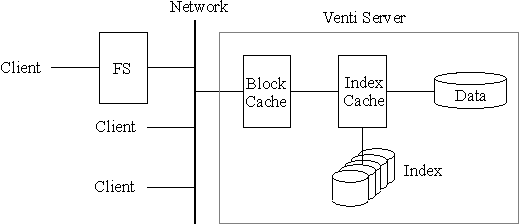
\includegraphics[scale=.7]{venti_prop}
\caption{\label{fig:venti} Venti network system and component setup.}
\end{center}
\end{figure}

\vspace*{-.2in}
\section{Method of Approach}
\label{sec:method}
\vspace*{-.1in}

In order to implement the proposed research, an open source server-side file manager will need to be acquired and extended. The file manager must be lightweight and compatible with the UNIX operating environment. To start, a database will be implemented so that it is able to hold a hashed key and the location of the file on the disk. An example of this schema can be seen in figure \ref{fig:schema}. The software, upon installation will run an initial scan of all files on the system in the specified upload folders. The file hash will be generated by running an SHA256 hashing function over each file currently on the disk. An INSERT will be run on the database for each file and will record the files current position on the disk, and it will record the result of the hash. Using the searching method outlined by the authors of the first paper in section \ref{sec:relatedwork}, the database will be searched for duplicate hash entries. When a duplicate entry is found, the file manager will remove all but the latest modified entry, and in place of the old modified files, a pointer will be implemented that links to the one remaining file.

In the case of needing duplicate files, so one can be modified while retaining the integrity of the original, it will be possible to open the original using the pointer, but if a saved copy of the file differs from the one that the pointer refers to, the pointer will be overwritten by the new file. This will allow the file system to work as it had before the file manager was implemented, retaining full intuitiveness and flexibility, but data redundancy can be avoided.

When a user uploads a file to the server using the web form, several methods are called. The first method called accepts the file through the submission dialogue and makes a hash using the hash function. The hash is then checked against all hashes currently in the database, if there is a match, a URL will be returned to the user of the same file that is currently in the database and the duplicate file is dropped. If the hash does not currently match an item in the database, the file is uploaded and stored in the submissions directory, then an insert is run with the location of the file on the disk, and the hash that was generated for the upload. Once the insert has successfully completed, a unique URL us generated from the primary key of the row that was just created, followed by a hyphen and the first 10 characters of the hash. This system would prevent other users from easily accessing files without a direct link as they would have to determine not only the $ID$ of the image, but also the first 10 digits of the files hash.

When a user accesses the file from the provided link, the system will run a query that looks up the ID and verifies the hash segment, if it is correct, the image location will be used to provide either a view of the file, or a download link. The user never notices a difference, but on the server side we have ensured file redundancy has been eliminated.

\begin{figure}
\begin{center}
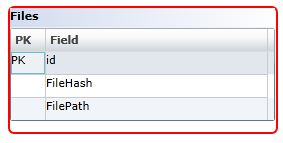
\includegraphics[scale=.8]{schema}
\caption{\label{fig:schema} Example schema to be used.}
\end{center}
\end{figure}

\vspace*{-.2in}
\section{Evaluation Strategy}
\label{sec:evaluate}
\vspace*{-.1in}

Evaluating the effectiveness of the program will entail several benchmark readings. The total number of files, the number of unique files, and the overall percentage of the disk will be evaluated to determine the effectiveness of the file manager. The total number of files will be fixed for every test run and the files used will be exactly the same for each run. The number of files will be the total number of files on the system located inside of the test file structure. This will not include program or system files. The number of duplicates will be randomly generated initially and the same file structure will be used each time the experiment is run. Duplicates are defined as files with identical meta-data and contents. The total disk space utilized will be determined by measuring the total size of the file structure containing the test structure.

Again, the same tests will be performed, but will be run with the proposed file management system. After the initial running of the program, statistics will be gathered that include the total run time of the program to completion, the final number of files, the number of remaining duplicate files, and the total storage space used. Because the system implements a text based database, the total storage space will be reduced, but the efficiency of the system will need to be determined.

\vspace*{-.1in}
\section{Research Schedule}
\label{sec:schedule}
\vspace*{-.1in}

The research schedule for the project is to be tentatively based off of the following deadlines. Due to the nature of the project and the wide array of pre-existing software required needing to be modified and implemented, unseen hurdles may arise. 

Phase 1 - 1 month: Find acceptable open source operating system and file manager. Begin the process of learning libraries and code so implementation can begin.

Phase 2 - 2-3 months: Develop a working program which is capable of satisfying the requirements outlined in section \ref{sec:method}. Set up a basic file structure to be used as a baseline for the research project. Record the number of files, number of duplicates, and the total storage space used compared to the file system with no user generated files.

Phase 3 - 1 week: During this time I will run various tests on the program using the proposed methods in section \ref{sec:method} and record the results of the experiment. After completion of initial file redundancy reduction, new files will be added to the collection, some unique, and others duplicate. The submissions directory on the server will be scanned for additional duplicates and ensure no false positives were denied. Results to be recorded are the final number of files, the number of remaining duplicates, and the total storage space used.

Phase 4 - remaining time: The results gathered throughout the test process will be evaluated and the software tweaked and finalized. After modifications are complete tests will be rerun and the final results will be evaluated.

\vspace*{-.1in}
\section{Conclusion}
\label{sec:conclusion}
\vspace*{-.1in}

With computers becoming ever more prevalent and data being generated at an exponential rate, it is becoming more and more necessary every day to reduce the redundancy and create a more efficient file system. By removing duplicate files from a system while retaining structure and organization this problem can be addressed and will not only reduce the amount of storage space required, but can also improve search efficiency by using stored information in a database and also reduce time spent sorting through structures manually removing duplicate data before backups. In addition, a significant amount of money can be saved due to the decrease in required storage space and backup costs.

\newpage

\bibliographystyle{plain}
\bibliography{senior_thesis_proposal}

\end{document}

